Per poter rilasciare sul mercato la nuova versione di ZConnect creata dopo le modifiche effettuate nella Sezione di Implementazione di questa tesi, Zucchetti S.P.A. ha affidato il compito di testare la migliorata funzionalità di monitoraggio delle presenze ad un team specifico di tester. Durante questo lavoro di tesi è stato seguito anche il team di tester, che tramite dei test funzionali ha validato la nuova versione di ZConnect. Le metodologie di test ed i risultati prodotti saranno rispettivamente descritti nelle Sezioni 5.1 e 5.2.

\section{Metodologia di test}
Durante questo lavoro di tesi, ho seguito anche il team di tester durante l'esecuzione dei test per poter rilasciare sul mercato la nuova versione di ZConnect. Il team di tester ha eseguito dei test funzionali. I test funzionali vengono utilizzati per individuare le discrepanze tra le specifiche e l'effettiva implementazione dei sistemi software \cite{TestFunzionali}. Tutti i test riportati di seguito sono stati eseguiti sia sulla versione Android che sulla versione iOS di ZConnect.

Inoltre, per far fronte al problema della frammentazione hardware e software tipico delle applicazioni per dispositivi mobili \cite{AndroidFragmentation}, tutti i test sono stati effettuati su dispositivi fisici con la versione minima e massima dei sistemi operativi per cui è sviluppata l'applicazione. In altre parole, è stato utilizzato un dispositivo Android con installata la versione 7 di Android e un dispositivo con installata la versione 13 di Android. Per iOS, è stato utilizzato un dispositivo fisico con installata la versione 14 di iOS e un dispositivo con installata la versione 16 di iOS. L'applicazione è stata testata anche su un tablet Android, poiché ZConnect è disponibile anche per tablet.

Il primo test funzionale eseguito è stato quello di apertura della mappa con un utente che ha associato numerose aree di lavoro per verificare che sulla mappa fossero presenti tutte le aree di lavoro, modellate tramite geofence, al cui centro fosse visibile un marker rosso che identifica il centro del geofence e che fosse visibile la posizione dell'utente identificata con un marker blu.

Successivamente è stato provato se cambiando la posizione dell'emulatore il marker dell'utente reagisse al cambio di posizione spostandosi a sua volta. Sono anche stati provati il pulsante per centrare la mappa sulla posizione dell'utente ed il pulsante per il ``follow-me", controllando che all'attivazione e alla disattivazione del ``follow-me" il pulsante cambi colore, in modo da dare un feedback adeguato all'utente. Con la funzionalità ``follow-me" attiva è stato provato a mettere l'app in background ed a riportala in foreground per verificare che la funzionalità rimanesse attiva. Infine è stato provato ad impostare, la modalità scura dell'app per vedere che i nuovi elementi grafici aggiunti alla mappa reagissero al cambiamento cambiando a loro volta colore. 


\begin{figure}[ht!]
    \begin{subfigure}{0.4\textwidth}
        \centering
        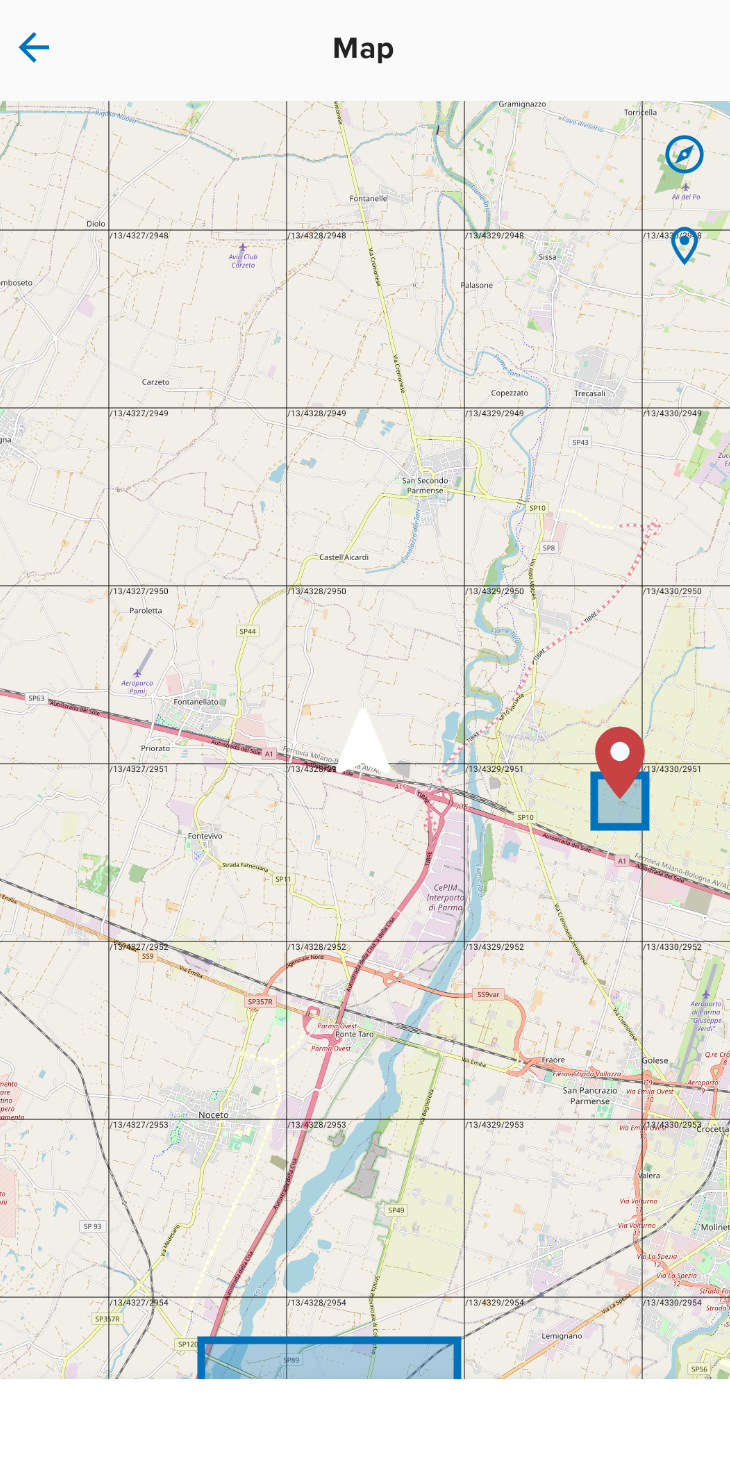
\includegraphics[width=\linewidth]{Immagini/zoom_dati_esempio.png}
        \caption{``follow-me" disattivo}
        \label{fig:vecchia_posizione_esterna_Android_2}
    \end{subfigure}
    \hspace{1cm} % Spazio orizzontale tra le immagini
    \begin{subfigure}{0.4\textwidth}
        \centering
        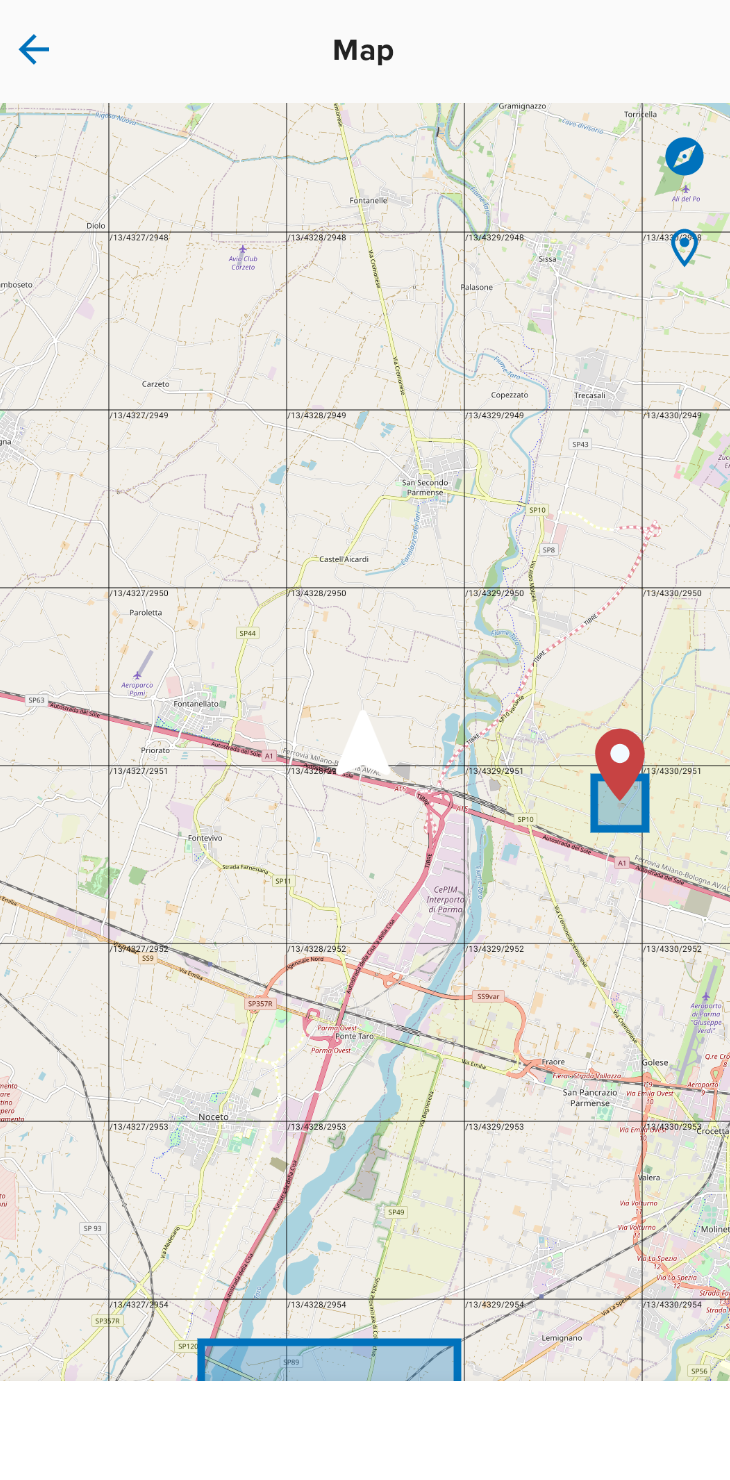
\includegraphics[width=\linewidth]{Immagini/follow_me_attivo.png}
        \caption{``follow-me" attivo}
        \label{fig:vecchia_posizione_interna_Android_2}
    \end{subfigure}
    \caption{Cambio del fill del bottone per attivare la funzione ``follow-me"}
    \label{fig:vecchia_mappa_android_3}
\end{figure}

Infine sono stati eseguiti dei test di non regressione. I test di non regressione vengono impiegati per verificare che le modifiche apportate al codice, gli aggiornamenti o le correzioni di errori non generino problemi alle funzionalità preesistenti dell'applicazione o del software, evitando nel contempo eventuali instabilità non correlate alle caratteristiche specifiche.
\' E stato provato ad effettuare una timbratura all'esterno ed all'interno di un area di lavoro associata all'utente, per verificare che nel caso della timbratura effettuata all'esterno dell'area di lavoro associata all'utente che questa venisse rifiutata, mentre nel caso di timbratura effettuata all'interno dell'area di lavoro associata all'utente che questa venisse accettata.
Infine è stato provata la visualizzazione della mappa sulla schermata delle timbrature passate, per testare che fosse ancora navigabile e che il luogo di lavoro dove è stata eseguita la timbratura fosse ancora visibile, modellato come un geofence.

\section{Risultati dei test}
I test funzionali illustrati nella Sezione 5.1 hanno prodotto per lo più risultati positivi.
\'E stato riscontrato un solo problema, che nella versione Android di ZConnect se viene attivata la funzionalità di ``follow-me" e successivamente, con la funzionalità attiva, l'applicazione viene messa in background e riportata in foreground, la funzionalità di ``follow-me" risulta non attiva. 

Grazie all'esecuzione di questi test funzionali è stato possibile individuare delle problematiche la cui risoluzione ha portato al rilascio di una versione di ZConnect funzionante e conforme alle specifiche descritte nella fase di analisi di questa tesi.